The implementation is performed in both Intel OpenMP runtime (iOMP) Version 20160322 and GNU Compiler Runtime (GOMP) version 6.1.0. 
we highlight the implementation and evaluation of some of the functions in Level 2 and 3: 
{\sf omp\_set\_wait\_policy}, {\sf omp\_quiesce} and {\sf omp\_thread\_create/exit/join}. 

For iOMP, the implementation of {\sf omp\_set\_wait\_policy} leverages the available 
implementation of suspending and resuming a thread used for the barrier implementation. Setting the 
wait policy of a thread to the {\sf SLEEP} policy is implemented by setting thread-specific variables. For
supporting changing policies to either {\sf SPIN} or {\sf YIELD}, the implementation needs to include codes for 
waking up those threads who are sleeping by using the provided thread suspension and resumption mechanisms.  
The thread suspension and resumption functionalities are implemented using pthread condition variable and mutex and 
we validate the effectiveness of our implementation by checking the kernel state of the program state when being 
executed.

\begin{table}[htbp]
	\centering
\begin{tabular}{|l|l|l|l|} \hline
\multicolumn{2}{|c|}{\textbf{Policy}} & \textbf{Description} & \textbf{Pseudo Code}\\ \hline
\multirow{2}{*}{ACTIVE} & SPIN\_BUSY  & User-level busy wait & while (!finished()) ;  \\ \cline{2-4}
                        & SPIN\_PAUSE & Busy wait with pausing CPU & while (!finished()) cpu\_relax(); \\ \hline
\multirow{2}{*}{PASSIVE}& SPIN\_YIELD & User-level busy wait &  while (!finished()) yield() ;  \\ \cline{2-4}
                      & SLEEP       & Thread sleeps. Others wake it up. & thread\_wait(); thread\_wake();\\ \hline
\end{tabular}
\label{table:implement_wait}
\caption{Implementation of wait policies }
\end{table}


\begin{comment}
\begin{tabular}{||c|c|c|c|c||} \hline  % l l r  --> three columns, 
\multirow{4}{*}{\rotatebox{90}{Impact}} & H &        &    &  \\ \cline{2-5}
       & M &        &    & \\ \cline{2-5}
       & L &        &    & \\ \cline{2-5}
       &  &    L    &  M   &  H \\ \hline
       & \multicolumn{4}{|c||}{\textbf{Probability}} \\ \hline
\end{tabular}



The thread behaves in the waiting state according to the policies specified by call to the {\sf omp\_set\_wait\_policy} or the default value from the wait-policy-var ICV. Below is the algorithm for the waiting loop.
\begin{algorithm}[ht]
	\small
    \caption{The waiting loop of threads that are not computing}

 \While{fork\_barrier\_not\_released}{
   thread\_state = omp\_thread\_state\_SPIN\;
   \If{unfinished tasks} {
	   execute\_task ( ... )\;
   }

   \If{program finished} {
	   break\;
   }

   \If{wait\_policy ==  omp\_thread\_state\_SPIN} {
	   continue\;
   }

   \If{wait\_policy ==  omp\_thread\_state\_YIELD} {
   	   thread\_state = omp\_thread\_state\_YIELD\;
	   spins = thread\_yield\_spin\_time\;
	   \While{program not finished and spins is greater than 0} {
		sched\_yield()\;
		spins -= 2\;
	   }
	   continue\;
   }
   thread\_state = omp\_thread\_state\_SLEEP\;
   thread\_suspend()\;

   
   \If{program finished} {
	   break\;
   }
   }
 \label{algo:worker_sched}
\end{algorithm} 

\end{comment}

The {\sf omp\_quiesce} implementation leverages the support for {\sf omp\_set\_wait\_policy} except that it 
should change the behavior of all the threads when it is called with SLEEP argument. 
%{\sf ACTIVE} and {\sf PASSIVE}
%environment setting for {\sf OMP\_WAIT\_POLICY} and the corresponding ICV, the use of turnaround and throughput mode for OpenMP execution, the 
%use of {\sf KMP\_BLOCKTIME} and {\sf kmp\_set\_blocktime} for setting the waiting time before putting a thread to sleep~\cite{iccmanual}, 
The implementation of {\sf omp\_quiesce(omp\_thread\_state\_KILL)} is a wrapper of 
the {\sf \_\_kmp\_internal\_end\_fini} internal API which shuts down the runtime system~\cite{iccmanual}. 


The implementation of  {\sf omp\_thread\_create/exit/join} needs to work around the need of a team when creating a thread, and the requirement 
of a fork barrier and join barrier when assigning any work to a thread in the runtime. An internal team object is created when creating a thread 
using the {\sf omp\_thread\_create} function. The implementation will first check the thread pool to find a waiting thread. If there is no thread
in the pool, it creates a native thread (PThread in Unix/Linux) launching into the runtime loop. The thread will be released for performing
user specified routine by the fork barrier. But it will skip the join barrier since it does not form a team with any other thread. 
The {\sf omp\_thread\_join} function is realized using a join counter. 

The total amount changes are about 200 lines of code, thus requiring small amount of efforts.  

\REM{
In general, to implement those four functions, we follow the three steps:
\begin{itemize}
	\item Define this function in file “kmp{\_}csupport.c”, 
	write down the implementation.
	\item Declare this function in file “kmp.h”, 
	using “KMP{\_}EXPORT” in front the declaration.
	\item Export this function in file “dllexports”, 
	assign a unique ID for this function.
\end{itemize}

\begin{enumerate}
	\item void omp{\_}quiesce()
	
	The purpose of this function is to shutdown or destroy all OpenMP threads in the thread pool. We have implemented it, as shown in Figure~\ref{omp:quiesce}, by using the Intel internal call to {\_}kmp{\_}internal{\_}end{\_}fini, which unloads the runtime library. Then, we have to register the master thread again so it can generate team of threads later when needed. This can be done by calling the {\_}kmp{\_}get{\_}global{\_}thread{\_}id{\_}reg( ).
	
	\begin{figure}
		\centering
		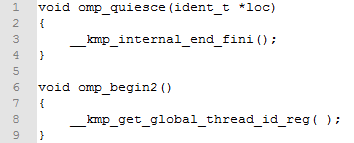
\includegraphics[width=0.7\textwidth] {images/omp_quisce}
		\caption{omp\_quiesce}
		\label{omp:quiesce}
	\end{figure}
	
	\item void omp{\_}set{\_}wait{\_}policy(PASSIVE \textbar ACTIVE)
	
	The idea of this function is to set the waiting thread behavior. PASSIVE value means that waiting threads should not consume CPU power while waiting. In other words, the OpenMP runtime system will put them into a sleep mode. On the other hand, ACTIVE value means that waiting threads should keep asking the CPU for work to do. The intention of doing this function is to measure the differences in performance between these different modes. 
	The implementation of this function is done by using the internal {\_}kmp{\_}stg{\_}parse{\_}wait{\_}policy as shown in Figure~\ref{omp:set_wait_policy}. The current OpenMP runtime system uses the library{\_}turnaround to indicate the ACTIVE mode and library{\_}throughput to indicate the PASSIVE mode. We pass an integer as its parameter. If it equals to 0, we set the wait policy to be passive, otherwise, active. We found a variable named “{\_}kmp{\_}library” in the environment setting file which has four different status for the waiting policy. So, we change this value accordingly, then we call a function “{\_}kmp{\_}aux{\_}set{\_}library” to set the changed value to the OpenMP environment.
	
	\begin{figure}
		\centering
		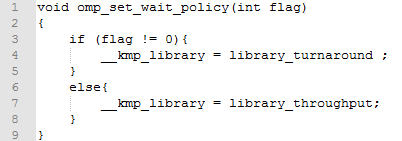
\includegraphics[width=0.7\textwidth] {images/omp_set_wait_policy}
		\caption{omp\_set\_wait\_policy}
		\label{omp:set_wait_policy}
	\end{figure}
	
	\item int omp{\_}thread{\_}create()
	
	The purpose of this function is to give the user the ability to create an OpenMP thread without using \#pragma omp parallel directive, and lets it be a user thread similar to pthread. The implementation of this function is shown in Figure~\ref{omp:create_thread}.
	So, we are creating one thread to execute the passed function. If there are enough available threads in the thread pool, we will get one thread from the thread pool and assign the task to it. If no thread is available in the thread pool, we create a new thread to execute this task, and then put the new thread back into the thread pool after completing its job. 
	
	\begin{figure}
		\centering
		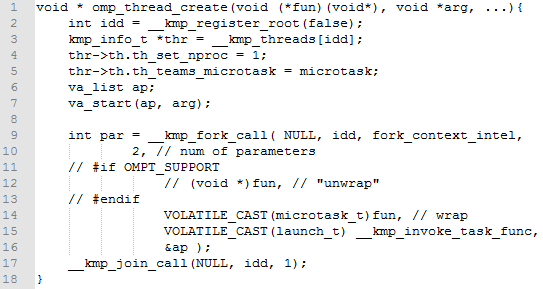
\includegraphics[width=0.7\textwidth] {images/omp_create_thread}
		\caption{omp\_create\_thread}
		\label{omp:create_thread}
	\end{figure}
	
\end{enumerate}
}
